\documentclass[aspectratio=169]{beamer}
\usetheme[block=fill]{metropolis}
\usepackage{tikz}
\usetikzlibrary{shapes.geometric, arrows.meta, positioning, calc}

\title{Building a Reproducible Scholarly Search Toolkit}
\subtitle{Episode 3: Persistent Identifiers (\texttt{ExternalIds})}
\author{Scholar Search Kit}
\date{}

\begin{document}

\begin{frame}[plain]
  \titlepage
\end{frame}

\begin{frame}{Episode Goal}
  \begin{alertblock}{The Goal}
    Build a unified \texttt{ExternalIds} model to track documents across multiple upstream providers.
  \end{alertblock}
  \vspace{0.5cm}
  A DOI from Crossref might look like \texttt{10.1000/182}, while from OpenAlex it might be \texttt{https://doi.org/10.1000/182}. We must normalize these to safely deduplicate records later.
\end{frame}

\begin{frame}{The Identifier Zoo}
  \begin{center}
  \resizebox{0.8\linewidth}{!}{
  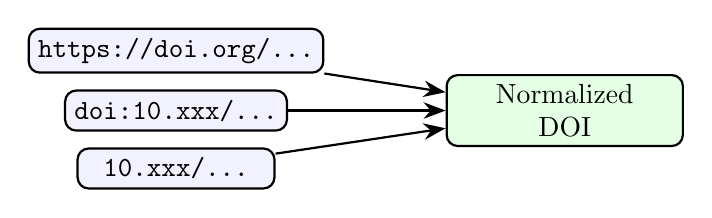
\begin{tikzpicture}[
      node distance=1.5cm and 2cm,
      box/.style={rectangle, draw, thick, rounded corners, minimum width=2.5cm, align=center, fill=blue!5},
      norm/.style={rectangle, draw, thick, rounded corners, minimum width=3cm, align=center, fill=green!10},
      arrow/.style={-{Stealth[scale=1.2]}, thick}
    ]
    
    \node[box] (doi1) {\texttt{https://doi.org/...}};
    \node[box, below=0.2cm of doi1] (doi2) {\texttt{doi:10.xxx/...}};
    \node[box, below=0.2cm of doi2] (doi3) {\texttt{10.xxx/...}};
    
    \node[norm, right=of doi2] (normalized) {Normalized\\DOI};
    
    \draw[arrow] (doi1) -- (normalized);
    \draw[arrow] (doi2) -- (normalized);
    \draw[arrow] (doi3) -- (normalized);
  \end{tikzpicture}
  }
  \end{center}
\end{frame}

\begin{frame}{The \texttt{ExternalIds} Dataclass}
  \begin{block}{Centralized Identity}
    We use a single dataclass to hold all known identities for a paper.
  \end{block}
  
  \begin{itemize}
      \item \texttt{doi}: The Digital Object Identifier (Normalized)
      \item \texttt{arxiv}: e.g., \texttt{2103.00020}
      \item \texttt{pubmed}: PubMed ID
      \item \texttt{openalex}: e.g., \texttt{W312...}
      \item \texttt{semantic\_scholar}: \texttt{CorpusId} or SHA
  \end{itemize}
\end{frame}

\begin{frame}{Implementation: Normalizing DOIs}
  \begin{block}{Regex to the Rescue}
    We strip prefixes (\texttt{https://doi.org/}, \texttt{doi:}) before storing.
  \end{block}
  
  \begin{itemize}
      \item Why? If Provider A returns a URL, and Provider B returns just the ID, a string comparison will fail.
      \item By normalizing to the bare \texttt{10.xxxx/...}, we guarantee that matching logic is foolproof.
  \end{itemize}
\end{frame}

\begin{frame}{Verification}
  \begin{alertblock}{Success Criteria}
    \begin{itemize}
        \item Initializing \texttt{ExternalIds} with a full URL DOI yields the stripped DOI.
        \item Two identical papers from different providers match perfectly on their \texttt{ExternalIds.doi}.
    \end{itemize}
  \end{alertblock}
\end{frame}

\end{document}
